%%%%%%%%%%%%%%%%%%%%%%%%%%%%%%%%%%%%%%%%%%%%%%%%%%%%%%%%%%%%%%%%%%%%%%%%%%%%%
\chapter{Evaluation}
\label{chap:evaluation}
Das Kapitel Evaluation zielt darauf ab, die entwickelten Lösungen und angewandten Methodiken einer umfassenden Bewertung zu unterziehen. Im Fokus steht dabei die Untersuchung, um eine Aussage zu treffen, ob die Hypothesen aus Kapitel \ref{sec:hypothesis} widerlegt oder bestätigt werden können. Diese Evaluierung stützt sich auf definierte Metriken und Benchmarks (siehe Kapitel \ref{sec:metrics}) innerhalb einer konfigurierten Testumgebung (siehe Kapitel \ref{subsec:testenv}), um objektive und reproduzierbare Ergebnisse zu erzielen. Die Ergebnisse werden anschließend im Kapitel \ref{sec:comparison} beurteilt und evaluiert.
%%%%%%%%%%%%%%%%%%%%%%%%%%%%%%%%%%%%%%%%%%%%%%%%%%%%%%%%%%%%%%%%%%%%%%%%%%%%%
\chapterstart

\section{Testumgebung, Testdaten und Metriken} \label{sec:metrics}
Dieses Kapitel befasst sich mit der Definition der Metriken, welche für die Beurteilung der Hypothesen von Relevanz sind. Die Testumgebung dient als Plattform für die Evaluierung und ist so konfiguriert, dass sie reproduzierbare Ergebnisse ermöglicht. In diesem Abschnitt werden die technischen Spezifikationen, die Auswahl der Werkzeuge und die Konfiguration der Umgebung detailliert beschrieben.
\subsection{Testumgebung} \label{subsec:testenv}
Die Evaluierung der Applikationen erfolgt in einer Cloud-nativen Umgebung, für die ein Kubernetes-Cluster als Testplattform dient. Für die Bereitstellung des Kubernetes-Clusters wird das Produkt ''Minikube'' \footnote{\url{https://minikube.sigs.k8s.io/docs/start/}} verwendet. Minikube ermöglicht die Einrichtung eines lokalen Kubernetes-Clusters auf einer einzelnen Maschine und bietet somit eine vereinfachte Plattform für Tests.

Die Host-Maschine für Minikube ist mit einem Intel i7-6700K Prozessor sowie 32 Gigabyte \ac{RAM} ausgestattet und läuft unter einem Debian-basierten Betriebssystem. Diese Konfiguration stellt die Grundlage für die Durchführung der Tests dar und gewährleistet die erforderliche Rechenkapazität sowie Kompatibilität mit der Kubernetes-Infrastruktur.
Durch die Verwendung von Minikube und der spezifizierten Hardware ist es möglich, einheitliche Testbedingungen zu gewährleisten. Dies erleichtert die Bewertung der Applikationsperformance und -skalierbarkeit unter definierten Bedingungen.

Um diese Testumgebung nun in einen testbaren Zustand zu bringen, wird ein Script für das Initialisieren des Minikube-Clusters geschaffen. Dieses Script, welches in Listing \ref{lst:minikubecreate} zu sehen ist, führt mit dem Befehl \lstinline{minikube create} ein Hochfahren des Clusters durch. Nach diesem Schritt werden alle notwendigen Plattform-Services bereitgestellt. Die Definitionen des Deployments dieser Plattform-Services, wie Datenbank und Message-Broker, sind in entsprechenden Konfigurationsdateien hinterlegt.
\newline
\begin{lstlisting}[language=Bash, caption={Script zur Erstellung des Minikube Clusters und dem Deployment der Plattform-Services.},label={lst:minikubecreate}]
#!/bin/sh

echo "Initializing Kubernetes cluster...\n"

minikube start --cpus 8 --memory 16g --driver docker --profile hypercrawler --kubernetes-version=v1.28.3

echo "Deploying platform services..."

kubectl apply -f services

sleep 5

echo "Waiting for MongoDB to be deployed..."

while [ $(kubectl get pod -l db=hypercrawler-mongo | wc -l) -eq 0 ] ; do
  sleep 5
done
...
\end{lstlisting}

\subsection{Datenerfassung und -speicherung}
Für die Erfassung und Speicherung der Metriken aus der Testumgebung wird Prometheus\footnote{\url{https://prometheus.io/}}, ein sogenanntes ''Monitoring-System'', eingesetzt. Prometheus fungiert als zentrales Element für das Monitoring, indem es Metriken von den Applikationen erfasst und persistiert. Diese Metriken werden daraufhin mithilfe eines Scripts abgefragt und in eine CSV-Datei geschrieben. Basierend auf diesen Daten können in weiterer Folge Analysen durchgeführt und Schlüsse gezogen werden. Die Daten werden unter anderem im GitHub-Projekt\footnote{\url{https://github.com/avollmaier/hypercrawler/tree/main/data}} gespeichert, um sie zugänglich zu machen.

Um diese Metriken zu sammeln, sind Konfigurationen in den Applikationen selbst notwendig. Die Applikationen bieten einen spezifischen Endpunkt \lstinline{http://<ip>:<port>/actuator/prometheus} an, der für die Erfassung der Metriken durch Prometheus vorgesehen ist. Dieser Endpunkt wird periodisch (Intervall von 1 Sekunde) von Prometheus abgefragt, wodurch eine fortlaufende und automatisierte Sammlung von Leistungsdaten ermöglicht wird. Die Integration dieses Endpunkts in die Applikationen erfolgt durch Hinzufügen der Abhängigkeit \lstinline{io.micrometer:micrometer-registry-prometheus} in der \lstinline{build.gradle}-Datei jedes Microservices. Dieser Schritt gewährleistet die Bereitstellung der Metriken in einem Format, das von Prometheus gelesen und verarbeitet werden kann. Verwendet wird für diese Anbindung das quelloffene Produkt Micrometer\footnote{\url{https://micrometer.io/}}. Das Ziel von Micrometer kann aus deren Produktdefintion entnommen werden:

\begin{spar}
\textit{Micrometer provides a facade for the most popular observability systems, allowing you to instrument your JVM-based application code without vendor lock-in.~\parencite[][]{micrometer}}
\end{spar}

\subsection{Beschreibung der Testdaten}\label{sec:testdaten}
Die Testdaten für den Crawling-Prozess bestehen aus realen Daten des \ac{WWW}. In \ref{subsec:datacollection} wird die Bedeutung der Diversität in der Größe der Testdaten hervorgehoben. Um die Reproduzierbarkeit der Ergebnisse zu gewährleisten, erfolgte kein Crawling von Live-Daten. Ein solches Vorgehen hätte variierende Ergebnisse zur Folge, bedingt durch Faktoren wie Netzwerklatenz. Daher beruht die Analyse auf statischen Datenquellen. Konkret umfasst sie Daten von Wikipedia, einer Online-Enzyklopädie. Bereitgestellt werden diese durch die Wikimedia Foundation.~\footnote{\url{https://dumps.wikimedia.org}}

Es werden für die Analyse der Hypothese \textit{\nameref{subsec:hypothesis:scalability}} drei statische HTML Auszüge verwendet:
\begin{itemize}
    \item Wikipedia Dump Sprache Tschuwaschisch [\textbf{Sprachkürzel nach ISO-639 CV}] \newline- Auszug vom 07.06 2008 20:30 mit einer Anzahl von 15835 HTML-Seiten \footnote{\url{https://dumps.wikimedia.org/other/static_html_dumps/current/cv/}}
    \item Wikipedia Dump Sprache Biharisch [\textbf{Sprachkürzel nach ISO-639 BH}]\newline- Auszug vom 07.06 2008 12:19 mit einer Anzahl von 4863 HTML-Seiten \footnote{\url{https://dumps.wikimedia.org/other/static_html_dumps/current/bh/}}
 \item Wikipedia Dump Sprache Amharisch [\textbf{Sprachkürzel nach ISO-639 AM}]\newline- Auszug vom 07.06 2008 09:33 mit einer Anzahl von 8618 HTML-Seiten \footnote{\url{https://dumps.wikimedia.org/other/static_html_dumps/current/am/}}
\end{itemize}

Für die Hypothese \textit{\nameref{subsec:hypothesis:ressource}} ist ein Datensatz ausreichend, da an diesem mehrere Tests durchgeführt werden. Verwendet wird hierzu folgender Datensatz:
\begin{itemize}
        \item Wikipedia Dump Sprache Armenisch [\textbf{Sprachkürzel nach ISO-639 HY}]\newline- Auszug vom 07.06 2008 10:46 mit einer Anzahl von 11461 HTML-Seiten \footnote{\url{https://dumps.wikimedia.org/other/static_html_dumps/current/hy/}}
\end{itemize}

Die statischen HTML-Inhalte sind über einen NGINX-Webserver\footnote{\url{https://www.nginx.com/}} zugänglich. Dieser Webserver, ebenso wie sämtliche andere Services, ist Teil der Testumgebung, beschrieben in Kapitel \ref{subsec:testenv}. Das Dockerfile des Docker-Images, dargestellt in Listing \ref{lst:dockernginx}, basiert auf dem offiziellen NGINX-Image. Es definiert auch die Übertragung der statischen Daten in das Image.

\begin{lstlisting}[language=Bash, caption={Dockerfile zur Erstellung des NGINX-Images, versorgt mit Testdaten.},label={lst:dockernginx}]
# Use a lightweight base image
FROM nginx:alpine

# Copy the static website files to the Nginx document root
COPY vo/ /usr/share/nginx/html

\end{lstlisting}
Durch die Ausführung des Befehls \lstinline{docker build -t <imageName> .} werden die Docker-Images, aufgeführt in Tabelle \ref{table:docker_images}, erstellt und sind anschließend verfügbar.

\begin{table}[H]
\centering
\begin{tabular}{|l|l|l|l|l|}
\hline
\textbf{REPOSITORY} & \textbf{TAG} & \textbf{IMAGE ID} & \textbf{CREATED} & \textbf{SIZE} \\ \hline
testdummy-hy & latest & c567e8e5a086 & 16 seconds ago & 255MB \\ \hline
testdummy-cv & latest & 4565997d5061 & 41 seconds ago & 275MB \\ \hline
testdummy-bh & latest & a7519e9f9854 & About a minute ago & 126MB \\ \hline
testdummy-am & latest & 39a4db98377d & About a minute ago & 149MB \\ \hline
\end{tabular}
\caption{Docker Images der Testdaten, bereitgestellt als NGINX-Docker-Image.}
\label{table:docker_images}
\end{table}


\subsection{Metriken zur Messung der Skalierbarkeit der Applikation} \label{}
Um eine Evaluierung der Skalierbarkeit durchzuführen, ist es notwendig die Metriken für die Messung zu definieren. Wie bereits in Abschnitt \ref{sec:method} erwähnt und in der Hypothese in Kapitel \ref{subsec:hypothesis:scalability} definiert, wird in dieser Arbeit die Skalierbarkeit anhand des Crawling-Durchsatzes bestimmt. Der Crawling-Durchsatz eines Webcrawlers, definiert als die Anzahl der in einem bestimmten Zeitraum verarbeiteten Webseiten, kann durch die folgende Formel (siehe \ref{form:durchsatzdefinition}) ausgedrückt werden:

\begin{equation}
    \text{Crawling-Durchsatz} = \frac{\text{Anzahl der verarbeiteten Webseiten}}{\text{Zeitraum}}
    \label{form:durchsatzdefinition}
\end{equation}

wobei der \textbf{Zeitraum} in \textbf{Sekunden} angegeben wird.\newline \newline
Diese Formel wird als Ausgangspunkt für die Evaluierung verwendet. Des Weiteren wird die Gesamtdauer des Crawling-Vorgangs protokolliert. Die Gesamtdauer wird ab dem Zeitpunkt gemessen, wo der Crawling-Prozess gestartet wird. Beendet wird die Messung bei einer vollständigen Untersuchung aller HTML-Seiten. Da die Anzahl der Seiten bekannt ist, kann eine klare Definition des Endes definiert werden. Beide Metriken werden infolgedessen mit einer monolythischen Softwarelösung verglichen.
\subsection{Metriken zur Effizienz von \acl{AOT}}\label{subsec:metrikefficience}
Für die Analyse von \ac{AOT} im Vergleich zu \ac{JIT} werden in der Hypothese \textit{\nameref{subsec:hypothesis:ressource}} folgende Metriken genannt:
\begin{enumerate}
    \item CPU-Nutzung der Applikation
    \item Arbeitsspeicherverbrauch der Applikation
    \item Die Zeit zwischen dem Start der Applikation und der ''Application Readiness'' (Zeitraum bis zu dem Punkt, an dem die Anwendung bereit ist, Anfragen zu bearbeiten)
\end{enumerate}

Die aktuelle CPU-Nutzung wird anhand der Metrik \lstinline{process_cpu_usage} von Prometheus analysiert. 
Für die Analyse des Arbeitsspeicherverbrauchs wird die Metrik \lstinline{jvm_memory_used_bytes} von Prometheus verwendet.

Für die Erfassung der Startzeit wird weder ein Actuator-Endpoint noch Prometheus verwendet. Stattdessen erfolgt die Untersuchung der Application Readiness durch die in Listing \ref{lst:readiness} dargestellte Anpassung. Dabei wird ein sogenannter ''Listener'' registriert, welcher Änderungen im Status der Application Readiness aufzeichnet und anschließend protokolliert. Mit dieser Methode lässt sich die Startzeit der Applikation, definiert als der Zeitraum bis zum Beginn der Annahme von Anfragen, im Bereich von Millisekunden erfassen.

\begin{lstlisting}[language=Java, caption={Code zur Analyse der Application Readiness am Beispiel des Crawler Services.},label={lst:readiness}]
@SpringBootApplication
public class CrawlerApplication {
  private static Long startTimeMillis;

  public static void main(String[] args) {
    startTimeMillis = System.currentTimeMillis();
    SpringApplication.run(CrawlerApplication.class, args);
  }

  @EventListener
  public void onEvent(AvailabilityChangeEvent<ReadinessState> event) {
    if (Objects.requireNonNull(event.getState()) == ReadinessState.ACCEPTING_TRAFFIC) {
      Long readinessMillis = System.currentTimeMillis();
      log.info("Readiness probe completed in {} ms", readinessMillis - startTimeMillis);
    }
  }
}
\end{lstlisting}
\newpage
\section{Evaluierung der Lösungen} \label{sec:comparison}
Das nachfolgende Kapitel hat das Ziel, die erzielten Ergebnisse zu präsentieren, zu evaluieren sowie die formulierten Hypothesen zu verifizieren oder zu falsifizieren. Im Unterkapitel \ref{sec:comparisonmicroservice} erfolgt die Untersuchung der Hypothese bezüglich der Skalierbarkeit (siehe Hypothese \textit{\nameref{subsec:hypothesis:scalability}}). Das Kapitel \ref{sec:comparisonaot} fokussiert sich auf die Überprüfung der Hypothese zur Ressourcennutzung (siehe Hypothese \textit{\nameref{subsec:hypothesis:ressource}}).
\subsection{Evaluierung der Microservice-Architektur hinsichtlich Skalierbarkeit}\label{sec:comparisonmicroservice}
Die Skalierbarkeitsanalyse erfolgte durch die Durchführung von drei Web-Crawling Durchläufen, die jeweils sowohl mit der Microservice als auch mit der Monolithischen Lösung durchgeführt wurden. Dabei wurde der Crawling-Durchsatz und die Gesamtdauer des Crawling-Vorgangs verglichen. Der Crawling-Durchsatz wurde für Zeitrahmen des gesamten Crawling-Prozesses betrachtet. Gemessen wurde ab dem Start des Crawling-Prozesses bis zur Persistierung der letzten HTML-Seite. Diese Zeit wurde in den Tabellen \ref{tab:scalability_analysis_micro} und \ref{tab:scalability_analysis_mono} protokolliert. \newline
Zur Analyse der monolithischen Anwendung wurde ein Java-Projekt erstellt, welches den Crawling-Prozess mithilfe der gleichen Mechanismen durchführt. Dieses Projekt ist im GitHub-Repository des Prototyps einsehbar.\footnote{\url{https://github.com/avollmaier/hypercrawler}}

Um den Zeitpunkt abzufragen, wann der Crawling-Prozess abgeschlossen ist, wurde ein Script erstellt, welches den Zeitpunkt des Starts und des Endes, also den Zeitpunkt ab dem alle Seiten persistiert wurden, misst. Dieses Script liefert die exakten Zeitstempel zurück, mit welchen infolgedessen eine Berechnung des Durchsatzes und der Durchlaufzeit stattfindet. Durch dieses Vorgehen kann die Unsicherheit des Messvorgangs mithilfe der Integration eines automatisierten Prozesses vermieden werden.\newline


\begin{table}[H]
\begin{tabular}{|l|l|l|l|}
\hline
\textbf{Datensatz}                                                      & \textbf{Seitenanzahl} & \textbf{Durchsatz (Seiten/Sekunde)} & \textbf{Durchlaufzeit} \\ \hline
\begin{tabular}[c]{@{}l@{}}Wikipedia Dump\\ Tschuwaschisch\end{tabular} & 15835                       & \textbf{63,09}                                   & \textbf{251 Sekunden}                       \\ \hline
\begin{tabular}[c]{@{}l@{}}Wikipedia Dump\\ Biharisch\end{tabular}      & 4863                             & \textbf{54,64}                                   & \textbf{89 Sekunden}                       \\ \hline
\begin{tabular}[c]{@{}l@{}}Wikipedia Dump\\ Amharisch\end{tabular}      & 8618                             & \textbf{62,45}                                   & \textbf{138 Sekunden}                       \\ \hline
\end{tabular}
\caption{Skalierbarkeitsanalyse des Crawling-Prozesses (Microservice Lösung).}
\label{tab:scalability_analysis_micro}
\end{table}

\begin{table}[H]
\begin{tabular}{|l|l|l|l|}
\hline
\textbf{Datensatz}                                                      & \textbf{Seitenanzahl} & \textbf{Durchsatz (Seiten/Sekunde)} & \textbf{Durchlaufzeit} \\ \hline
\begin{tabular}[c]{@{}l@{}}Wikipedia Dump\\ Tschuwaschisch\end{tabular} & 15835                            & \textbf{50,91}                                   & \textbf{311 Sekunden}                       \\ \hline
\begin{tabular}[c]{@{}l@{}}Wikipedia Dump\\ Biharisch\end{tabular}      & 4863                             & \textbf{51,73}                                   & \textbf{94 Sekunden}                       \\ \hline
\begin{tabular}[c]{@{}l@{}}Wikipedia Dump\\ Amharisch\end{tabular}      & 8618                             & \textbf{50,1}                                   & \textbf{172 Sekunden}                       \\ \hline
\end{tabular}
\caption{Skalierbarkeitsanalyse des Crawling-Prozesses (Monolythische Lösung).}
\label{tab:scalability_analysis_mono}
\end{table}

\textbf{Durchschnittlicher Durchsatz für die Microservice Lösung}\newline
Aus Tabelle \ref{tab:scalability_analysis_micro} werden nun die Durschnittswerte für den Crawling-Durchsatz in der Einheit \textit{Seiten pro Sekunde} berechnet. Diese Berechnung ist in Gleichung \ref{eq:microservice_durchsatz} ersichtlich. 
\begin{equation}
\frac{63,09 + 54,64 + 62,45}{3} = 60,06
\label{eq:microservice_durchsatz}
\end{equation}

\textbf{Durchschnittlicher Durchsatz für die Monolithische Lösung}\newline
Des weiteren wurde der durchschnittliche Durchsatz der Monolythischen Anwendungen mithilfe der Daten aus Tabelle \ref{tab:scalability_analysis_mono} berechnet. Dies ist in Gleichung \ref{eq:monolith_durchsatz} ersichtlich.
\begin{equation}
\frac{50,91 + 51,73 + 50,1}{3} = 50,91
\label{eq:monolith_durchsatz}
\end{equation}

Die Verbesserung in Prozent berechnet sich wie folgt (siehe Gleichung \ref{eq:verbesserung_prozent}):
\begin{equation}
\text{Verbesserung (\%)} = \left( \frac{\text{Neuer Durchsatz} - \text{Alter Durchsatz}}{\text{Alter Durchsatz}} \right) \times 100
\label{eq:verbesserung_prozent}
\end{equation}
\newpage
Setzt man diese Werte in die Formel ein, so erhält man das nachfolgende Ergebnis, wie in Gleichung \ref{eq:verbesserung_prozent_rechnung} ersichtlich:
\begin{equation}
\text{Verbesserung (\%)} = \left( \frac{60,06 - 50,91}{50,91} \right) \times 100 = \left( \frac{9,15}{50,91} \right) \times 100 \approx 17,95\%
\label{eq:verbesserung_prozent_rechnung}
\end{equation}

Die Verbesserung in der Durchsatzleistung beträgt 17,95\%.
Des Weiteren zeigt die Analyse, dass während des Crawling-Durchlaufs (Datensatz Wikipedia Dump Tschuwaschisch Microservice) ein Service nicht in der Lage war, alle Nachrichten zu beantworten, was zu deren Anhäufung führte. Es existiert somit ein Flaschenhals, vor allem bei großen Datensätzen. Wie in der Abbildung \ref{fig:rabbitmq} ersichtlich ist, warten \textbf{3495 Nachrichten} in der Message-Queue. In dieser Situation ist es möglich, den Vorteil zu nutzen, dass eine weitere Instanz dieses Services hochgefahren werden kann, um die Last auf beide Instanzen zu verteilen. So kann ein noch höherer Durchsatz erzeugt werden, da genau bestimmt wird, welche Komponente einen Engpass verursacht. Somit ist eine gezieltere Steuerung als bei einer Monolythischen Lösung möglich. Diese Instanz kann durchaus auch auf einer anderen Maschine laufen, was eine geographische Verteiltheit ermöglicht.
\begin{figure}[H]
    \centering
    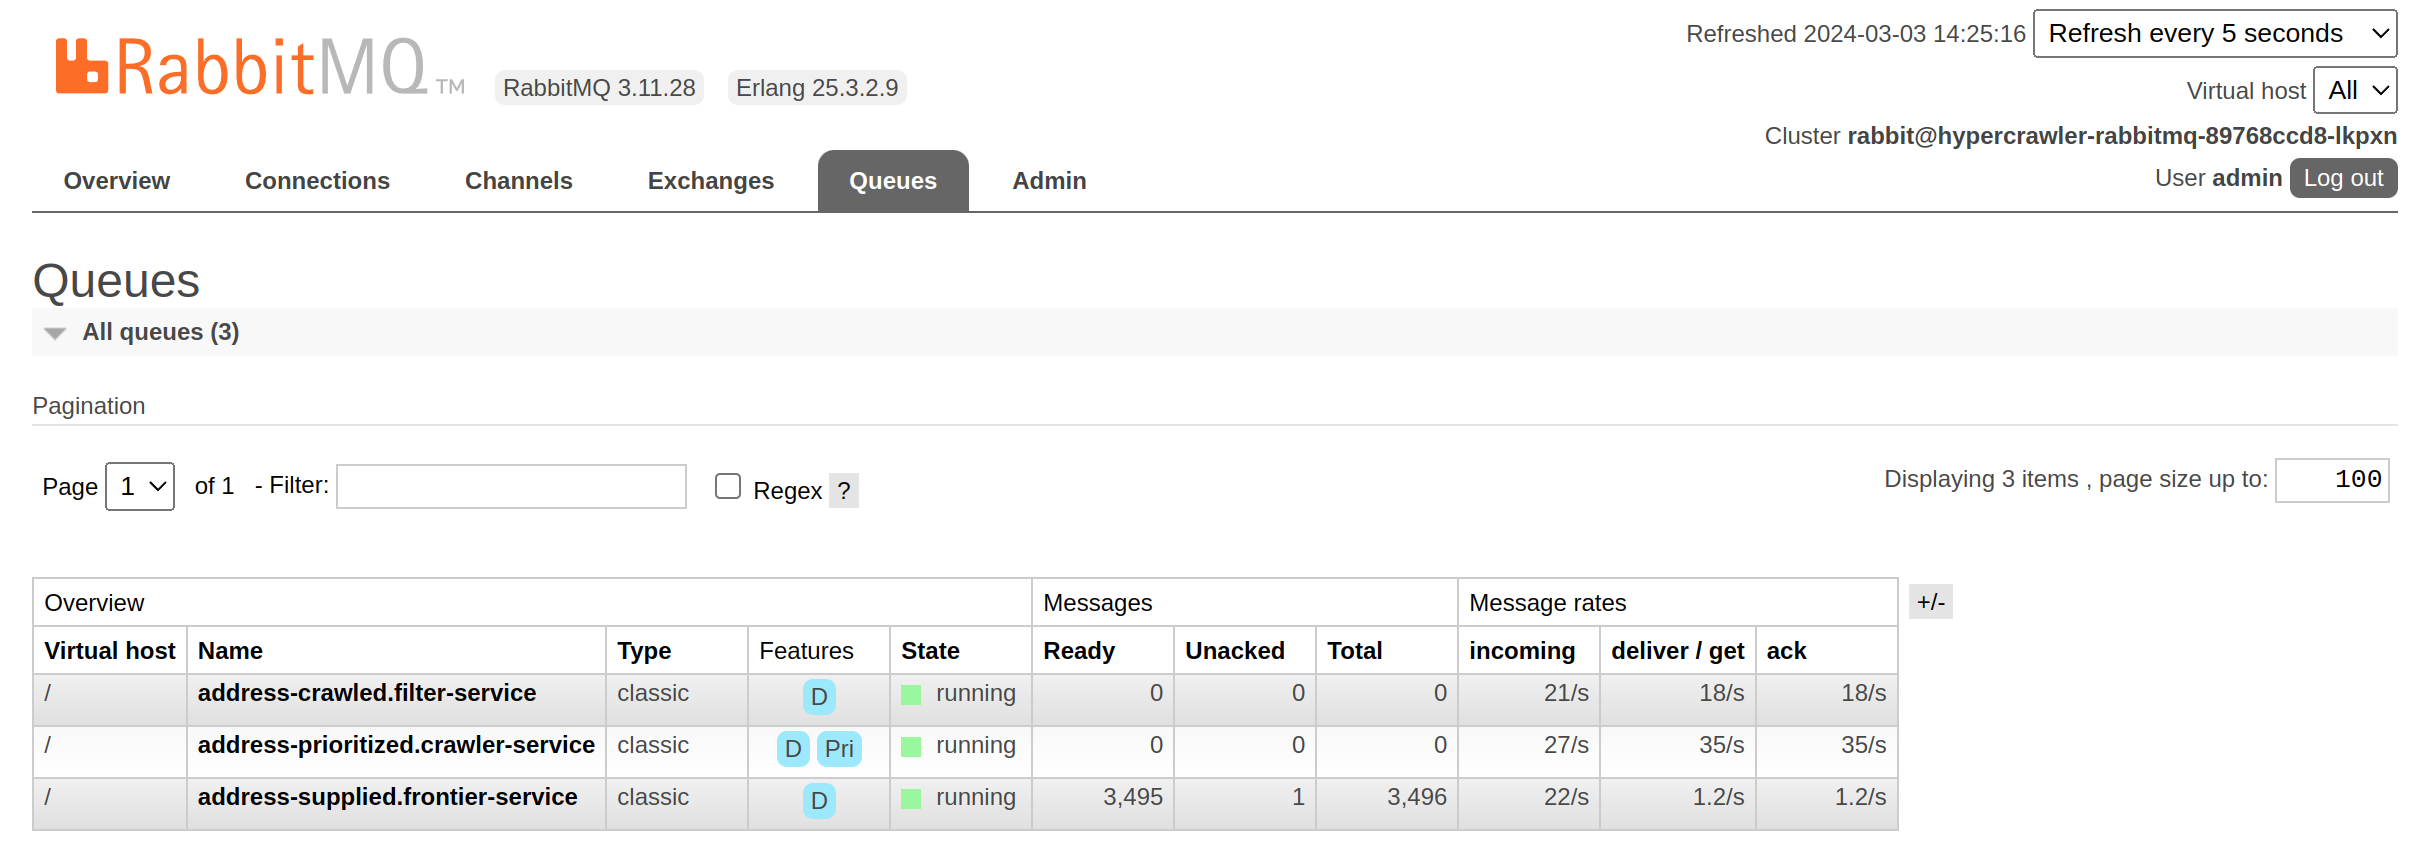
\includegraphics[width=14cm]{images/80_eval/Screenshot from 2024-03-03 14-25-29.png}
    \caption[]{Darstellung der RabbitMQ-Message-Queue mit 3495 unbearbeiteten Nachrichten.}
    \label{fig:rabbitmq}
\end{figure}
\newpage
\subsection{Evaluierung der Verbesserungen der Effizienz durch \acl{AOT}.} \label{sec:comparisonaot}
In diesem Abschnitt wird die CPU-Nutzung und der Speicherverbrauch eines Services untersucht.  Hierzu wird ein Crawling-Vorgang mit beiden Technologien gestartet und danach werden mithilfe von Prometheus die Daten abgefragt. Als Testset wird die statische Webseite von Wikipedia in der Armenischen Sprache verwendet. Damit vergleichbare Werte möglich sind, wurden in beiden Crawling-Prozessen die Werte des \textbf{Crawling Service} abgefragt.  \newline\newline
\textbf{Vergleich der CPU-Nutzung}\newline
Die nachfolgende Abbildung \ref{fig:cpujit} zeigt die CPU-Nutzung in Prozent über den gemessenen Zeitraum. Zu sehen ist die Analyse mit \ac{JIT}-Artefakten. Die Kennwerte für die CPU-Nutzung wurden analysiert wobei folgende Ergebnisse ersichtlich wurden:
\begin{enumerate}
    \item Maximale CPU-Nutzung: 23,5\%
    \item Durchschnittliche CPU-Nutzung: 5,29\%
\end{enumerate}

\begin{figure}[H]
    \centering
    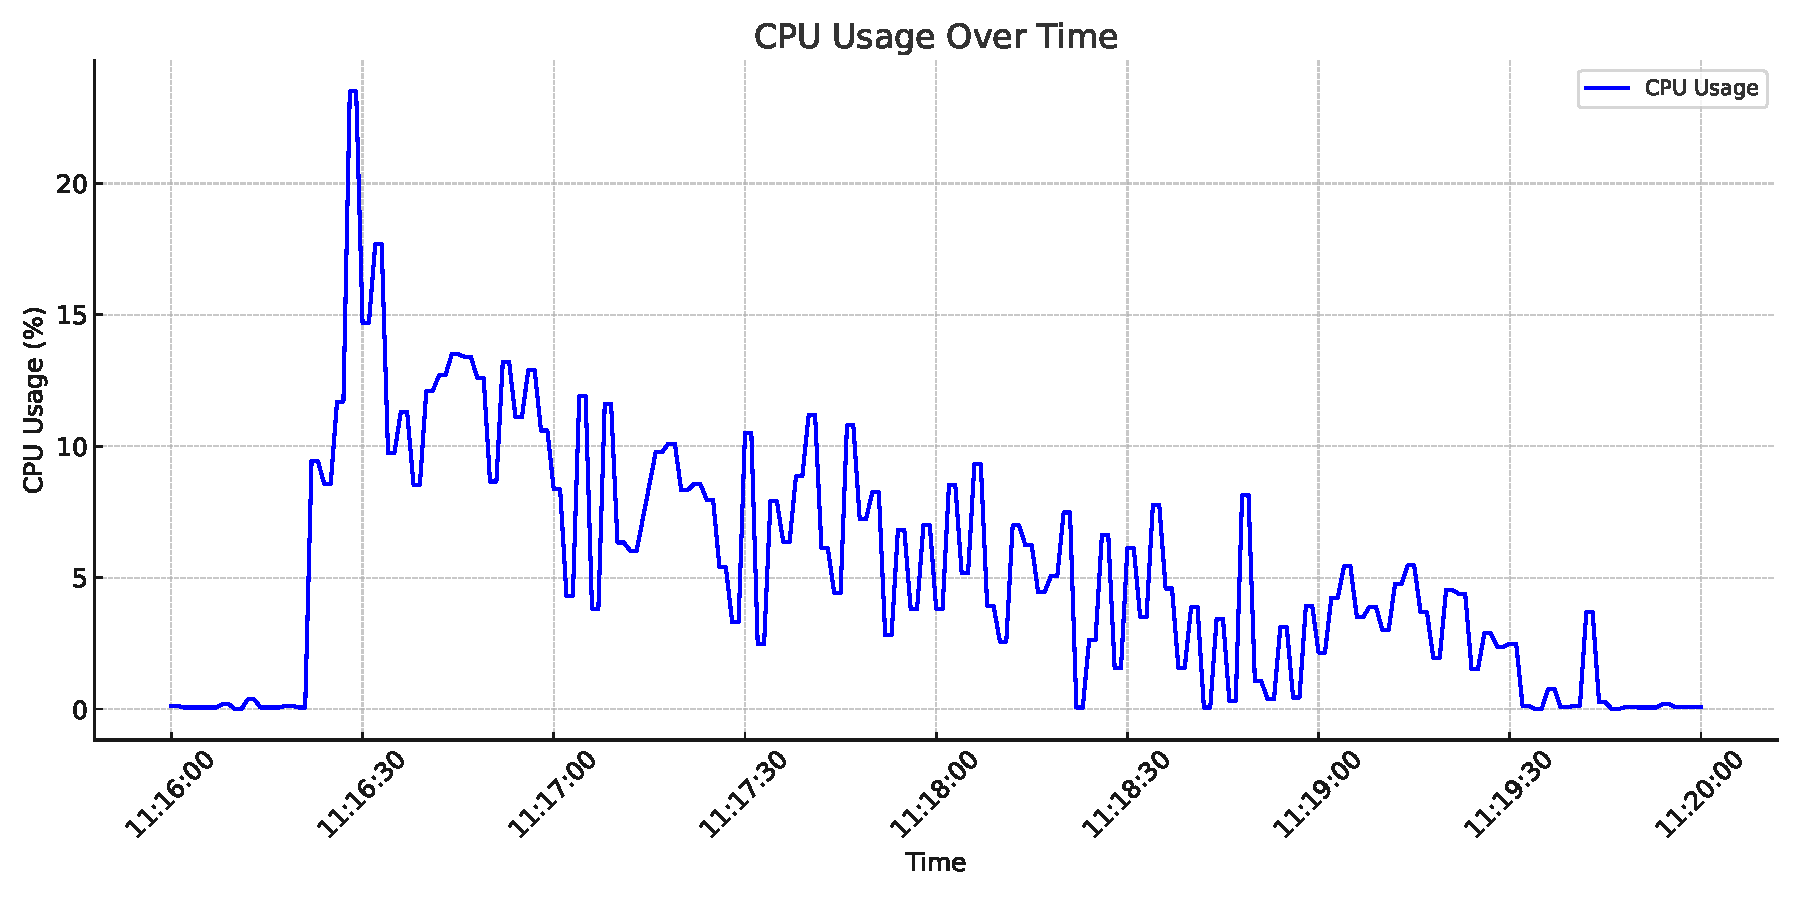
\includegraphics[width=12cm]{images/80_eval/CPU_Usage_Over_Time.pdf}
    \caption[]{Darstellung der CSV-Daten der CPU-Nutzung als Diagramm mit \acl{JIT}.}
    \label{fig:cpujit}
\end{figure}
Die Abbildung \ref{fig:cpuaot} zeigt nun die CPU-Nutzung in Prozent, jedoch mit \ac{AOT}-Artefakten. Aus diesen Daten lassen sich folgende Kennwerte ableiten:
\begin{enumerate}
    \item Maximale CPU-Nutzung: 8,5\%
    \item Durchschnittliche CPU-Nutzung: 2,24\%
\end{enumerate}
\begin{figure}[H]
    \centering
    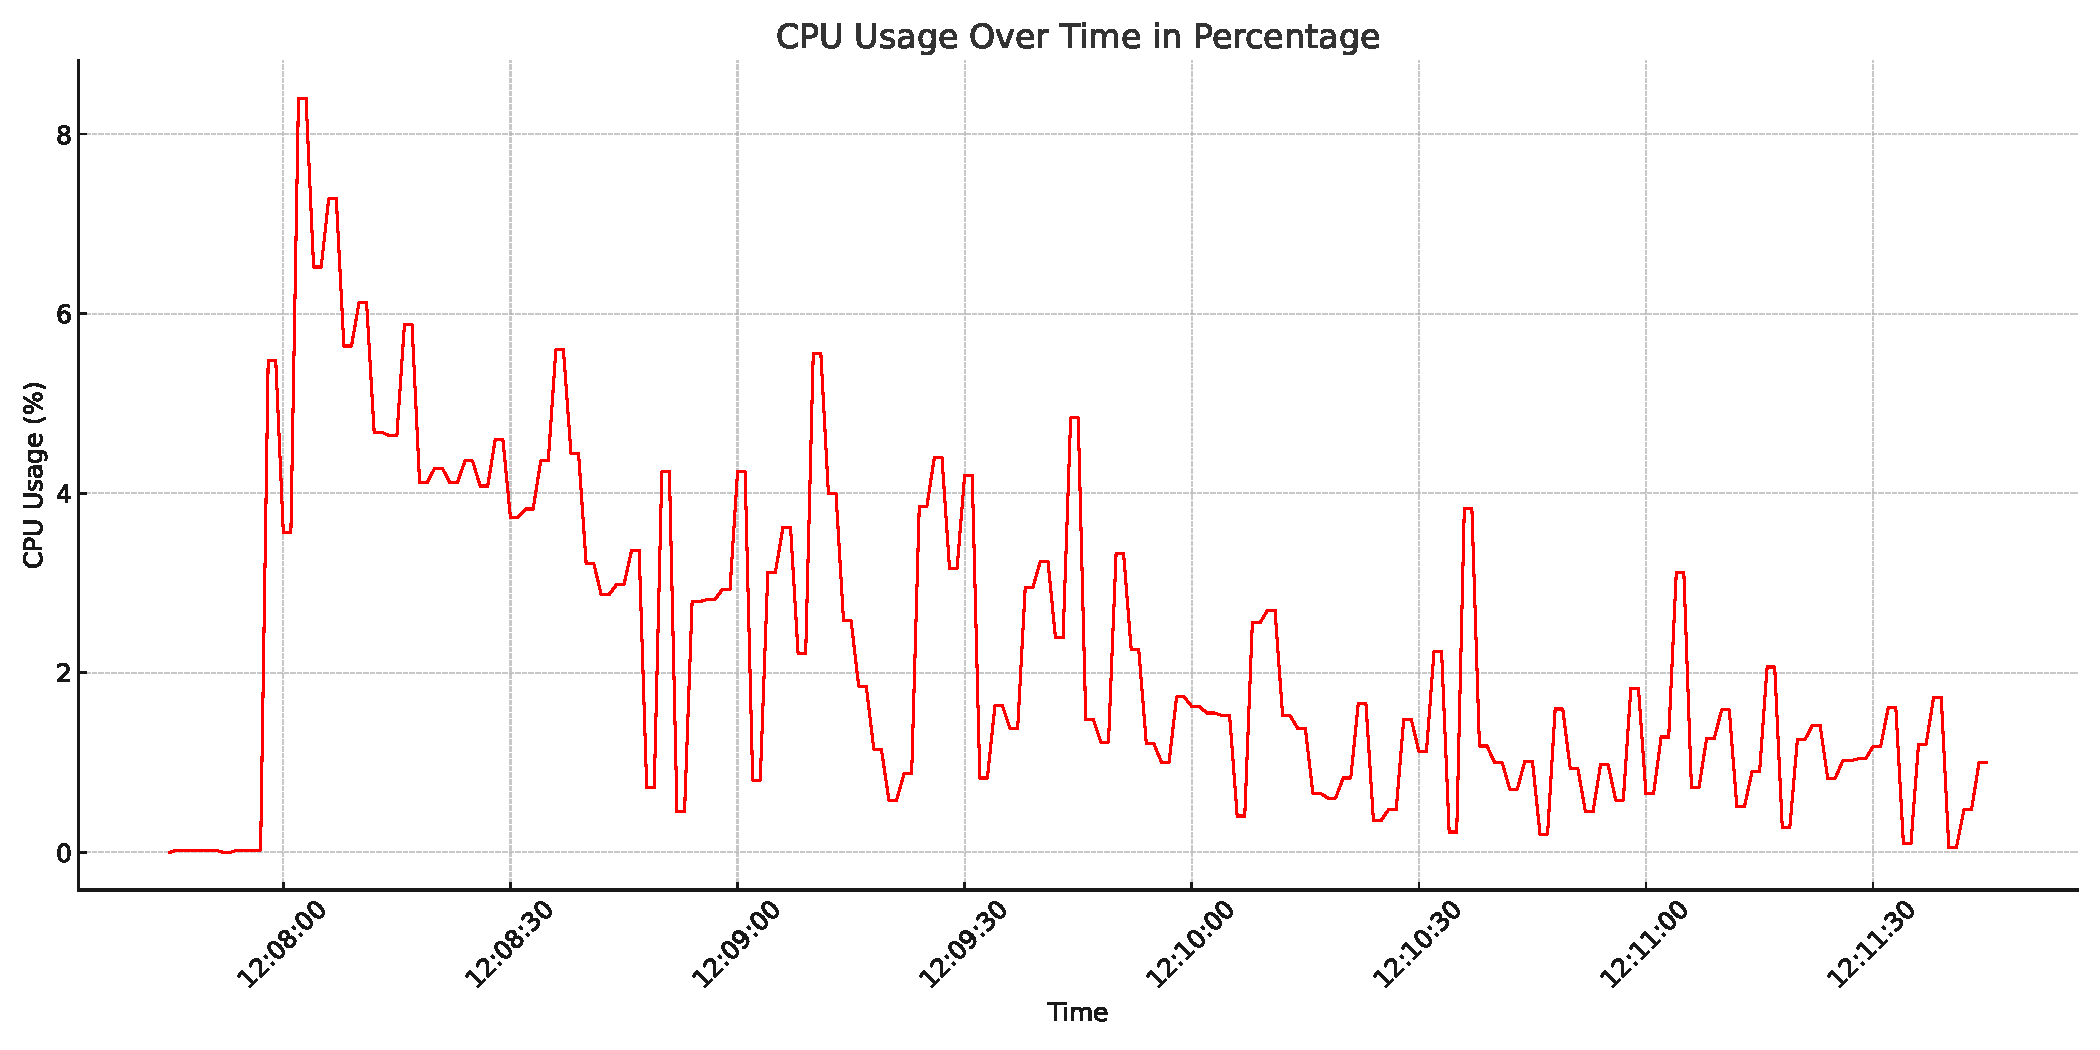
\includegraphics[width=12cm]{images/80_eval/cpu_usage_percentage_simplified_over_time.pdf}
    \caption[]{Darstellung der CSV-Daten der CPU-Nutzung als Diagramm mit \acl{AOT}.}
    \label{fig:cpuaot}
\end{figure}
\textbf{Ergebnisse der Berechnung} \newline
Die \ac{AOT}-Kompilierung zeigt im Vergleich zur \ac{JIT}-Kompilierung eine deutliche Verbesserung in Bezug auf die CPU-Nutzung: \ac{AOT}-Artefakte des Crawler-Service haben in diesem Test eine um 63,8\% geringere maximale CPU-Nutzung als \ac{JIT}-Artefakte des gleichen Serives. Die durchschnittliche CPU-Nutzung der \ac{AOT}-Artefakte ist in diesem Test auch um 57,65\% geringer als mit \ac{JIT}-Artefakte. Diese Berechnung erfolgt anhand der Formel \ref{eq:jitspuc}:
\begin{equation}
\text{Verbesserung (\%)} = \left( \frac{\text{AOT CPU-Nutzung} - \text{JIT CPU-Nutzung}}{\text{JIT CPU-Nutzung}} \right) \times 100    
\label{eq:jitspuc}
\end{equation}

Für die Überprüfung der Hypothese, dass \ac{AOT} eine 20\%ige Verbesserung der CPU-Nutzung gegenüber \ac{JIT} bietet, soll die Differenz im Vergleich zu \ac{JIT} betrachtet werden, da \ac{JIT} der Ausgangspunkt oder der ''vorherige Zustand'' ist und \ac{AOT} der ''verbesserte Zustand''. Diese Formel gilt auch für die Analyse der Speicherauslastung.

Diese Ergebnisse zeigen, dass die \ac{AOT}-Kompilierung in diesem Szenario erheblich effizienter in Bezug auf die CPU-Nutzung ist, als die \ac{JIT}-Kompilierung. Die Hypothese der CPU-Nutzung ist somit verifiziert.\newline \newline
\textbf{Vergleich der Speicher-Nutzung}\newline
Die Abbildung \ref{fig:memjit} zeigt die Nutzung des Arbeitsspeichers über den bestimmten Zeitraum, dargestellt in Megabyte. Die X-Achse der Abbildung stellt die Zeit in regelmäßigen Intervallen dar, während die Y-Achse die Nutzung des Arbeitsspeichers in Megabyte angibt.
Durch die Analyse der Daten wurde festgestellt, dass der durchschnittliche und maximale Nutzungswert wie folgt lautet:
\begin{enumerate}
    \item Maximaler Nutzungswert: 760.75 Megabyte
    \item Durchschnittliche Nutzungswert: 433.70 Megabyte
\end{enumerate}
\begin{figure}[H]
    \centering
    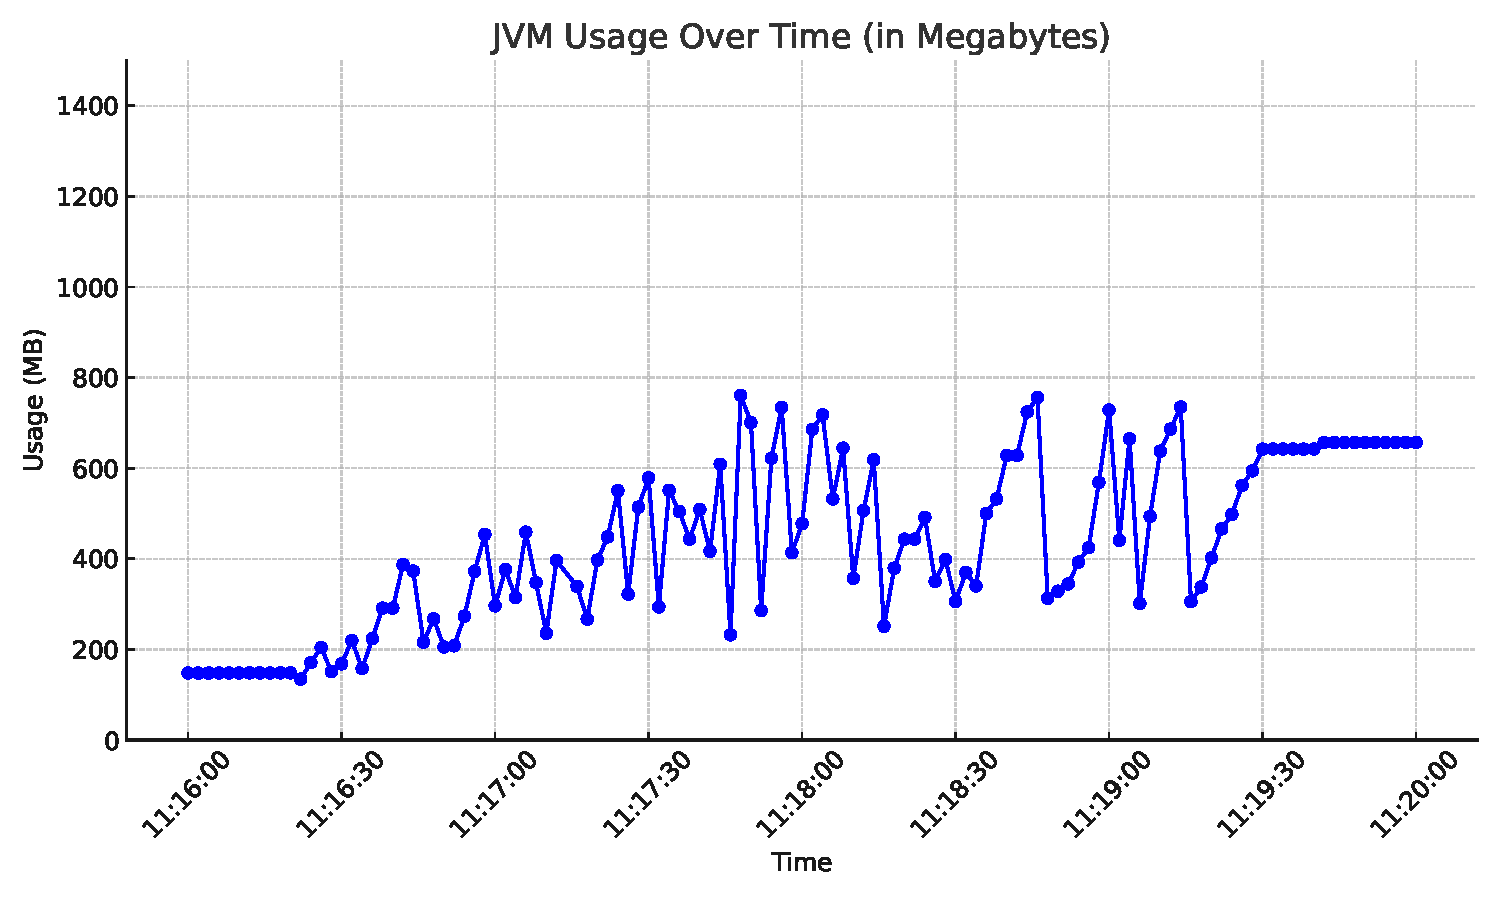
\includegraphics[width=12cm]{images/80_eval/JVM_Usage_Timeseries_MB_1500.pdf}
    \caption[]{Darstellung der CSV-Daten des Speicherverbrauchs als Diagramm mit \acl{JIT}.}
    \label{fig:memjit}
\end{figure}

Außerdem wurde eine Analyse mit \ac{AOT}-Artefakten durchgeführt. Die Abbildung \ref{fig:memaot} zeigt den Verlauf des Speicherverbrauchs. Folgende Kennzahlen lassen sich aus den Daten ableiten:
\begin{enumerate}
    \item Maximaler Nutzungswert: 156,78 Megabyte
    \item Durchschnittliche Nutzungswert: 78.075 Megabyte
\end{enumerate}

\begin{figure}[H]
    \centering
    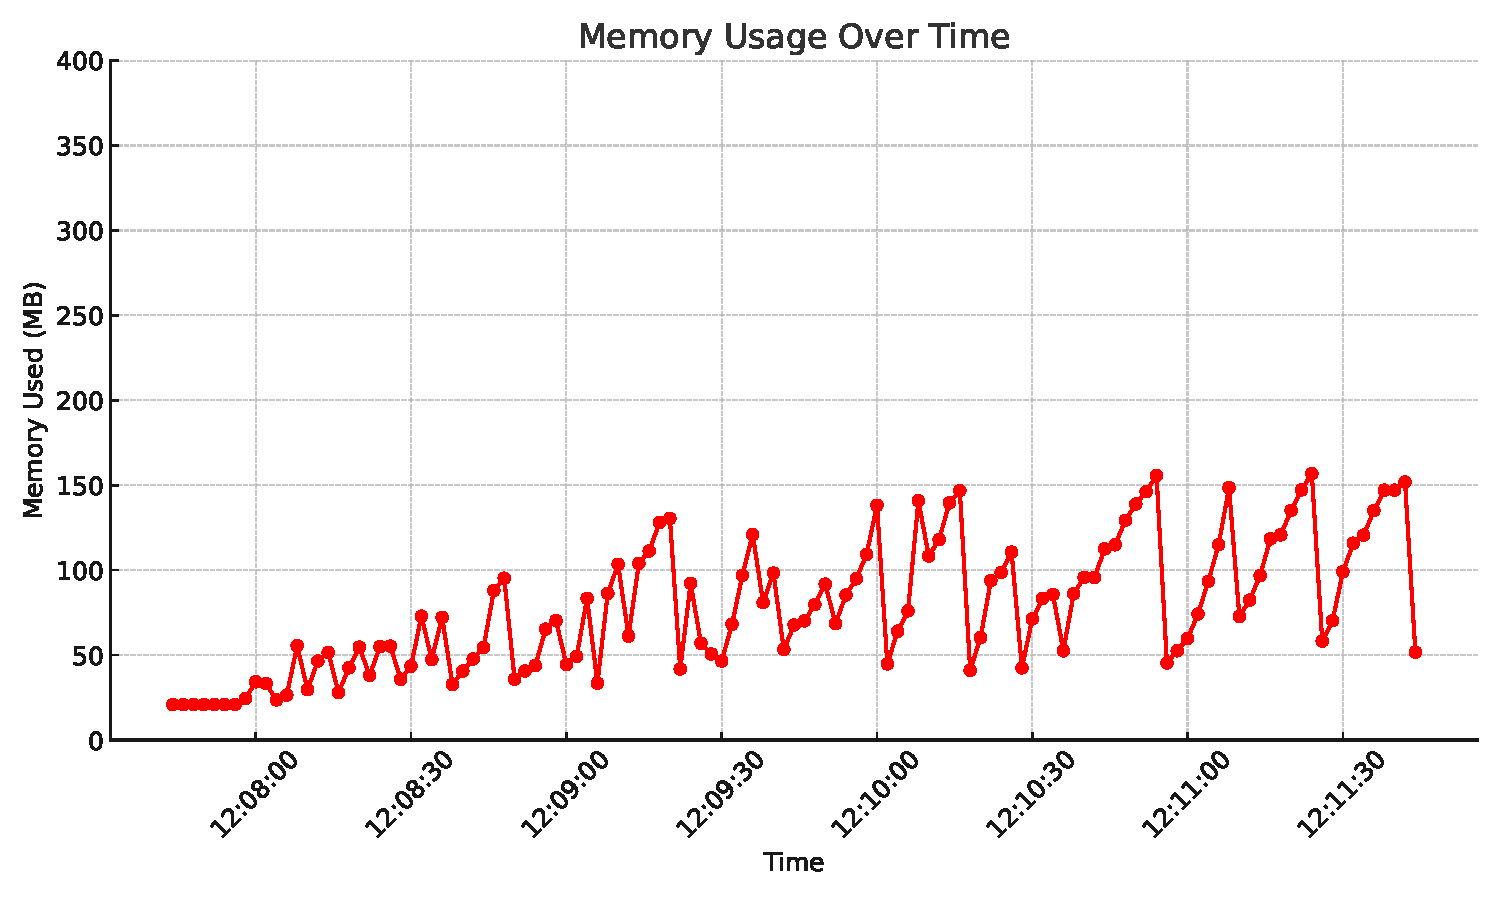
\includegraphics[width=12cm]{images/80_eval/memory_usage_over_time_very_final.pdf}
    \caption[]{Darstellung der CSV-Daten des Speicherverbrauchs als Diagramm mit \acl{AOT}.}
    \label{fig:memaot}
\end{figure}
\textbf{Ergebnisse der Berechnung} \newline
Aus den zuvor aufgestellten Berechnungen lassen sich folgende Verbesserungen ableiten: Für den maximalen Nutzungswert \textbf{79.39\%} und für den durchschnittlichen Nutzungswert \textbf{82.00\%}.

Durch diese Kennzahlen lässt sich ebenfalls eine Optimierung im Bereich des Speicherverbrauchs bestätigen. Folglich ist auch der Aspekt der Hypothese bezüglich der Speichernutzung verifiziert.

\textbf{Vergleich der Startzeit der Anwendungen}\newline
Bei der Durchführung der Lasttests wurden von allen vier Services die Startzeiten analysiert. Einmal mit \ac{AOT} und einmal mit \ac{JIT}. Diese wurden gegenübergestellt und verglichen. Die Startzeiten der \ac{JIT}-Artefakte ist in \ref{tab:startzeitjit} zu sehen.
\begin{table}[H]
\centering
\begin{tabular}{|l|l|l|l|l|}
\hline
\textbf{Anwendung}     & \textbf{Test 1 (ms)} & \textbf{Test 2 (ms)} & \textbf{Test 3 (ms)} & \textbf{Test 4 (ms)} \\ \hline
\multirow{1}{*}{Manager-Service}  & 4526 & 4277 & 4151 & 3916 \\ \hline
\multirow{1}{*}{Frontier-Service}        & 5285 & 5259 & 4567 & 4530 \\ \hline
\multirow{1}{*}{Crawler-Service}         & 4415 & 4587 & 4567 & 4668 \\ \hline
\multirow{1}{*}{Filter-Service}          & 3845 & 3904 & 3818 & 3733 \\ \hline
\end{tabular}
\caption{Startzeit der JIT-Anwendungen bis zur Application Readiness.}
\label{tab:startzeitjit}
\end{table}

Die Artefakte, kompiliert mit \ac{AOT}, wurden den gleichen Tests unterzogen, wie zuvor erwähnt. Die Ergebnisse sind in Tabelle \ref{tab:startzeitaot} protokolliert.
\begin{table}[H]
\centering
\begin{tabular}{|l|l|l|l|l|}
\hline
\textbf{Anwendung}     & \textbf{Test 1 (ms)} & \textbf{Test 2 (ms)} & \textbf{Test 3 (ms)} & \textbf{Test 4 (ms)} \\ \hline
\multirow{1}{*}{Manager-Service}  & 293 & 346 & 558 & 514 \\ \hline
\multirow{1}{*}{Frontier-Service}        & 460 & 277 & 361 & 634 \\ \hline
\multirow{1}{*}{Crawler-Service}         & 298 & 334 & 358 & 712 \\ \hline
\multirow{1}{*}{Filter-Service}          & 461 & 272 & 374 & 379 \\ \hline
\end{tabular}
\caption{Startzeit der AOT-Anwendungen bis zur Application Readiness.}
\label{tab:startzeitaot}
\end{table}
Nach der Analyse wurden die Durchschnittszeiten (nach Formel \ref{equ:startzeiten}) für jeden Service berechnet. Dabei wurden die durchschnittlichen Startzeiten für jede Anwendung unter Verwendung unterschiedlicher Technologien ermittelt. Die Ergebnisse sind in Tabelle \ref{table:druch} protokolliert.
\begin{equation}
\text{Durchschnitt} = \frac{\sum \text{Startzeiten}}{\text{Anzahl der Tests}}    
 \label{equ:startzeiten}
\end{equation}

\begin{table}[H]
\centering
\begin{tabular}{|l|l|l|}
\hline
\textbf{Anwendung}        & \textbf{JIT Durchschnitt (ms)} & \textbf{AOT Durchschnitt (ms)} \\ \hline
Manager-Service  & 4217.5                & 427.75                \\ \hline
Frontier-Service & 4910.25               & 433                   \\ \hline
Crawler-Service  & 4559.25               & 425.5                 \\ \hline
Filter-Service   & 3825                  & 371.5                 \\ \hline
\end{tabular}
\caption{Durchschnittliche Startzeiten von JIT- und AOT-Kompilierung.}
\label{table:druch}
\end{table}
Infolgedessen wird die prozentuale Verringerung der Startzeiten durch \ac{AOT} im Vergleich zu \ac{JIT} mit der Formel \ref{equat:jitdurchschnitt} berechnet:
\begin{equation}
    \text{Prozentuale Verringerung} = \left( \frac{\text{AOT Durchschnitt} - \text{JIT Durchschnitt}}{\text{JIT Durchschnitt}} \right) \times 100\%
\label{equat:jitdurchschnitt}
\end{equation}

Berechnung der prozentualen Verringerung der Startzeit des Manager Service:
\[
\left( \frac{427.75 - 4217.5}{4217.5} \right) \times 100 = \left( \frac{-3789.75}{4217.5} \right) \times 100 \approx -89.86\%
\]

Berechnung der prozentualen Verringerung der Startzeit des Frontier Service:
\[
\left( \frac{433 - 4910.25}{4910.25} \right) \times 100 = \left( \frac{-4477.25}{4910.25} \right) \times 100 \approx -91.18\%
\]

Berechnung der prozentualen Verringerung der Startzeit des Crawler Service:
\[
\left( \frac{425.5 - 4559.25}{4559.25} \right) \times 100 = \left( \frac{-4133.75}{4559.25} \right) \times 100 \approx -90.67\%
\]
Berechnung der prozentualen Verringerung der Startzeit des Filter Service:
\[
\left( \frac{371.5 - 3825}{3825} \right) \times 100 = \left( \frac{-3453.5}{3825} \right) \times 100 \approx -90.29\%
\]
Hierbei ist zu erwähnen, dass das negative Vorzeichen vor den jeweiligen Ergebnissen der Berechnung aufzeigt, dass eine tatsächliche Verringerung stattgefunden hat.
Diese Berechnungen zeigen, dass die Verwendung von \ac{AOT}-Artefakten im Vergleich zu \ac{JIT}-Artefakten eine erhebliche Verbesserung der Startzeiten für die Anwendungen ermöglicht. Die Prozentsätze stellen die Verringerung dar und verdeutlichen, wie viel schneller die Anwendungen mit \ac{AOT} im Vergleich zu \ac{JIT} sind. Die Hypothese \ref{subsec:hypothesis:ressource} ist somit vollständig verifiziert.

Ein wesentlicher Nachteil, welcher betrachtet werden muss, sind aber die höheren Build-Zeiten. So lässt sich aus folgendem Auszug (siehe Listing \ref{lst:buildzeitenaot}), welcher den Build-Prozess des Manager Services repräsentiert, eine hohe Buildzeit von \textbf{346,3 Sekunden} ableiten. Um die gesamte Zeit für die Initialisierung des Prozesses zu berechnen, addieren man die Zeiten für jeden Schritt der \ac{AOT}-Kompilierung:
\[
8.3s + 118.3s + 54.2s + 25.0s + 10.8s + 103.1s + 11.1s + 15.5s = 346.3s
\]
Die gesamte Zeit beträgt also \textbf{346.3 Sekunden}. 

\begin{lstlisting}[language=Bash, caption={Auszug des AOT-Build-Prozesses mit der Darstellung der Build-Zeiten.},label={lst:buildzeitenaot}]
    [creator]     [1/8] Initializing...                   (8.3s @ 0.21GB)
    [creator]     [2/8] Performing analysis...  [*******] (118.3s @ 2.71GB)
    [creator]       25,851 (91.86%) of 28,143 types reachable
    [creator]       41,516 (67.82%) of 61,217 fields reachable
    [creator]      121,759 (64.21%) of 189,635 methods reachable
    [creator]     [3/8] Building universe...              (54.2s @ 2.45GB)
    [creator]     [4/8] Parsing methods...      [*****]   (25.0s @ 2.48GB)
    [creator]     [5/8] Inlining methods...     [***]     (10.8s @ 3.71GB)
    [creator]     [6/8] Compiling methods...    [*******] (103.1s @ 6.05GB)
    [creator]     [7/8] Layouting methods...    [***]     (11.1s @ 4.29GB)
    [creator]     [8/8] Creating image...       [****]    (15.5s @ 5.44GB)
\end{lstlisting}
\chapterend
